\documentclass{article}

\usepackage{fancyhdr}
\usepackage{extramarks}
\usepackage{amsmath}
\usepackage{amsthm}
\usepackage{amsfonts}
\usepackage{amssymb}
\usepackage{tikz}
\usepackage[plain]{algorithm}
\usepackage{algpseudocode}
\usepackage{fitch}

\usetikzlibrary{automata,positioning}

%
% Basic Document Settings
%

\topmargin=-0.45in
\evensidemargin=0in
\oddsidemargin=0in
\textwidth=6.5in
\textheight=9.0in
\headsep=0.25in

\linespread{1.1}

\pagestyle{fancy}
\lhead{\hmwkAuthorName}
\chead{\hmwkClass\ (\hmwkClassInstructor\ | \hmwkClassTime): \hmwkTitle}
\rhead{\firstxmark}
\lfoot{\lastxmark}
\cfoot{\thepage}

\renewcommand\headrulewidth{0.4pt}
\renewcommand\footrulewidth{0.4pt}

\setlength\parindent{0pt}

%
% Create Problem Sections
%

\newcommand{\enterProblemHeader}[1]{
    \nobreak\extramarks{}{Problem \arabic{#1} continued on next page\ldots}\nobreak{}
    \nobreak\extramarks{Problem \arabic{#1} (continued)}{Problem \arabic{#1} continued on next page\ldots}\nobreak{}
}

\newcommand{\exitProblemHeader}[1]{
    \nobreak\extramarks{Problem \arabic{#1} (continued)}{Problem \arabic{#1} continued on next page\ldots}\nobreak{}
    \stepcounter{#1}
    \nobreak\extramarks{Problem \arabic{#1}}{}\nobreak{}
}

\setcounter{secnumdepth}{0}
\newcounter{partCounter}
\newcounter{homeworkProblemCounter}
\setcounter{homeworkProblemCounter}{1}
\nobreak\extramarks{Problem \arabic{homeworkProblemCounter}}{}\nobreak{}

%
% Homework Problem Environment
%
% This environment takes an optional argument. When given, it will adjust the
% problem counter. This is useful for when the problems given for your
% assignment aren't sequential. See the last 3 problems of this template for an
% example.
%
\newenvironment{homeworkProblem}[1][-1]{
    \ifnum#1>0
        \setcounter{homeworkProblemCounter}{#1}
    \fi
    \section{Problem \arabic{homeworkProblemCounter}}
    \setcounter{partCounter}{1}
    \enterProblemHeader{homeworkProblemCounter}
}{
    \exitProblemHeader{homeworkProblemCounter}
}

%
% Homework Details
%   - Title
%   - Due date
%   - Class
%   - Section/Time
%   - Instructor
%   - Author
%

\newcommand{\hmwkTitle}{Homework\ \#3}
\newcommand{\hmwkDueDate}{October 6, 2016}
\newcommand{\hmwkClass}{CS204}
\newcommand{\hmwkClassTime}{Section A}
\newcommand{\hmwkClassInstructor}{Prof. Sungwon Kang}
\newcommand{\hmwkAuthorName}{Ohjun Kwon}

%
% Title Page
%

\title{
    \vspace{2in}
    \textmd{\textbf{\hmwkClass:\ \hmwkTitle}}\\
    \normalsize\vspace{0.1in}\small{Due\ on\ \hmwkDueDate\ at 11:59pm}\\
    \vspace{0.1in}\large{\textit{\hmwkClassInstructor\ | \hmwkClassTime}}
    \vspace{3in}
}

\author{\textbf{20160051 \hmwkAuthorName}}
\date{}

\renewcommand{\part}[1]{\textbf{\large Part \Alph{partCounter}}\stepcounter{partCounter}\\}

%
% Various Helper Commands
%

% Useful for algorithms
\newcommand{\alg}[1]{\textsc{\bfseries \footnotesize #1}}

% For derivatives
\newcommand{\deriv}[1]{\frac{\mathrm{d}}{\mathrm{d}x} (#1)}

% For partial derivatives
\newcommand{\pderiv}[2]{\frac{\partial}{\partial #1} (#2)}

% Integral dx
\newcommand{\dx}{\mathrm{d}x}

% Alias for the Solution section header
\newcommand{\solution}{\textbf{\large Solution}}

% Probability commands: Expectation, Variance, Covariance, Bias
\newcommand{\E}{\mathrm{E}}
\newcommand{\Var}{\mathrm{Var}}
\newcommand{\Cov}{\mathrm{Cov}}
\newcommand{\Bias}{\mathrm{Bias}}

\begin{document}

\maketitle

\pagebreak

\begin{homeworkProblem}
\textbf{(a)}

$3\cdot 1+5\cdot 5=3+25=28=7k$ for $k=4$

$\therefore 1\triangleleft 5$

$3\cdot 3+5\cdot 1=9+5=14=7k$ for $k=2$

$\therefore 3\triangleleft 1$

$3\cdot 0+5\cdot 7=0+35=35=7k$ for $k=5$

$\therefore 0\triangleleft 7$\\

\textbf{(b)}

For $a=1$, $b=5$, $c=3$, $d=1$,

$1\triangleleft 5$ and $3\triangleleft 1$ are true as we shown in \textbf{(a)}.

$a\cdot c\triangleleft b\cdot d=1\cdot 3\triangleleft 5\cdot 1=3\triangleleft 5$

$3\cdot 3+5\cdot 5=9+25=34$ which is not a multiple of 7.

$3\triangleleft 5$ is false.
\end{homeworkProblem}

\begin{homeworkProblem}
The conclusion \textbf{(a)} is vaild. A word "if" in the definitions means if and only if, which means that the two statements are equivalent. However, a word "if" in the theorems establishes only one way. For example, in given statements, if $\triangle ABC$ is scalene, then all of the sides of $\triangle ABC$ have different lengths by the definition. On the other hand, we are not guaranteed that $\triangle ABC$ is a right triangle that is not isosceles, because the theorem gives us only the fact that if a triangle is right triangle that is not isosceles then a triangle is scalene.
\end{homeworkProblem}

\begin{homeworkProblem}
\textbf{(a)}
$\forall n\exists x\exists y\exists zP(n,x,y,z)$\\

\textbf{(b)}
\begin{align}
\lnot\forall n\exists x\exists y\exists zP(n,x,y,z)&\Leftrightarrow \exists n\lnot\exists x\exists y\exists zP(n,x,y,z)\\
&\Leftrightarrow \exists n\forall x\lnot\exists y\exists zP(n,x,y,z)\\
&\Leftrightarrow \exists n\forall x\forall y\lnot\exists zP(n,x,y,z)\\
&\Leftrightarrow \exists n\forall x\forall y\forall z\lnot P(n,x,y,z)
\end{align}
(1): universal negation\\
(2): existential negation\\
(3): existential negation\\
(4): existential negation\\

\textbf{(c)}
In order to give a counterexample for this statement, we have to give an example that satisfies \textbf{(b)}, i.e. we need to find some positive integer $n$ that is $x^n+y^n\neq z^n$ for any positive integers $x$, $y$, $z$.
\end{homeworkProblem}

\begin{homeworkProblem}
\textbf{(a)}
If x is a borfin, then x has been schlumpfed.

\textbf{(b)}
If x is not a borfin, then x has not been schlumpfed.

\textbf{(c)}
\textbf{(b)} is logically equivalent to the given theorem. We cannot tell anything about the converse of the theorem, but we can guarantee that the contrapositive is true if the given theorem is true. We can check this via making a truth table.
\begin{table}[ht!]
	\centering
	\begin{tabular}{c | c || c | c }
		$p$ & $q$ & $p\to q$ & $\lnot q\to \lnot p$ \\
		\hline
		T & T & T & T \\
		T & F & F & F \\
		F & T & T & T \\
		F & F & T & T
	\end{tabular}
	\caption{truth table}
	\label{tab:1}
\end{table}
\end{homeworkProblem}

\begin{homeworkProblem}
Yes. Triangles can exist in four-point geometry. We can find several triangles in a diagram(Figure~\ref{fig:1}) which satisfies all of the axioms from the four-point geometry. For example, in figure~\ref{fig:1}, we can find a triangle made of three points $x$, $y$, and $z$.
\begin{figure}[!ht]
	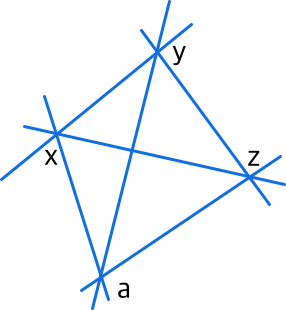
\includegraphics[width=0.3\textwidth]{four-point}
	\centering
	\caption{an example}
	\label{fig:1}
\end{figure}
\end{homeworkProblem}

\begin{homeworkProblem}
$a|b\Leftrightarrow \exists k$ s.t. $b=ka$\\
$b|c\Leftrightarrow \exists l$ s.t. $c=lb$\\
$\exists m$ s.t. $c=lb=l(ka)=(lk)a=ma$\\
$\therefore a|c$
\end{homeworkProblem}

\begin{homeworkProblem}
\textbf{(a)}
$n=5$\\
$n^2+2n=5\cdot 5+2\cdot 5=25+10=35$\\
3 does not divide 35.\\

\textbf{(b)}
$3|n\Leftrightarrow \exists k$ s.t. $n=3k$\\
$n^2+2n=(3k)^2+2(3k)=9k^2+6k=3(3k^2+2k)=3l$\\
$\exists l$ s.t. $n^2+2n=3l$\\
$\therefore 3|(n^2+2n)$
\end{homeworkProblem}

\begin{homeworkProblem}
$a, b\in \mathbb{Q}$\\
$\exists q, p ,r, s \in \mathbb{Z}$ ($p\neq 0, s\neq 0$) s.t. $a=\frac q p$, $b=\frac s r$\\
$\displaystyle a+b=\frac q p+\frac s r=\frac{qr+ps}{pr}\in \mathbb{Q}$\\
$\therefore a+b\in \mathbb{Q}$
\end{homeworkProblem}

\begin{homeworkProblem}
By the third statement of the Badda-Bing axiomatic system, if $x$ and $y$ are distinct baddas each hitting bing $q$, then there are no other bings hit by both $x$ and $y$. However, in our case, there are two distinct bings that are hit by $x$ and $y$, so it means that the baddas $x$ and $y$ are not distinct. Otherwise, it will not satisfy the axiom. Therefore, two baddas $x$ and $y$ are same. \qedsymbol
\end{homeworkProblem}

\begin{homeworkProblem}
Negate the conclusion: $\lnot ((a\notin v)\lor (b\notin v))$\\
$\lnot ((a\notin v)\lor (b\notin v))\Leftrightarrow \lnot (a\notin v)\land \lnot (b\notin v)\Leftrightarrow a\in v\land b\in v$\\
If $a$ and $b$ are distinct points, then there is a \textbf{unique} line $u$ by the first statement in the axiomatic system for four-point geometry. However, the line $v$, which is distinct from the line $u$, also contains two points $a$ and $b$, and it contradicts the uniqueness of the line. \qedsymbol
\end{homeworkProblem}
\end{document}